\chapter{Non-parametric methods}
\label{chap-nonparametric}

Neural networks have adaptable complexity, in the sense that we can
try different structural models and use cross validation to find one
that works well on our data.  Beyond neural networks, we may further
broaden the class of models that we can fit to our data, for example
as illustrated by the techniques introduced in this chapter.

Here, we turn to models that automatically adapt their complexity to
the training data.  The name {\em non-parametric
    methods}\index{non-parametric methods} is misleading: it is really a
class of methods that does not have a fixed parameterization in
advance.  Rather, the complexity of the parameterization can grow as
we acquire more data.

Some non-parametric models, such as nearest-neighbor, rely directly on the
data to make predictions and do not compute a model that summarizes
the data. Other non-parametric methods, such as decision trees\note{These are sometimes called {\em classification trees}; the decision analysis literature uses ``decision tree'' for a structure that lays out possible future events that consist of choices interspersed with chance nodes.},
can be seen as
dynamically constructing something that ends up looking like a more
traditional parametric model, but where the actual training data
affects exactly what the form of the model will be.

The non-parametric methods we consider here tend to have the form of a
composition of simple models:
\begin{itemize}
  \item{\em Nearest neighbor models}: (Section~\ref{sec-np_nn}) where we
        don't process data at training time, but do all the work when making
        predictions, by looking for the closest training example(s) to a given
        new data point.\index{nearest neighbor models}
  \item {\em Tree models}: (Section~\ref{sec-np_trees}) where we
        partition the input space and use different simple predictions on
        different regions of the space; the hypothesis space can become
        arbitrarily large allowing finer and finer partitions of the
        input space.\index{tree models}
  \item {\em Ensemble models}: (Section~\ref{sec-np_bagging}) in which
        we train several different classifiers on the whole space and
        average the answers; this decreases the estimation
        error.\index{ensemble models} In particular, we will look at
        bootstrap aggregation, or {\em bagging} of trees.
  \item{\em Boosting}\index{boosting} is a way to construct a model
        composed of a sequence of component models (e.g., a model consisting of
        a sequence of trees, each subsequent tree seeking to correct
        errors in the previous trees) that decreases both estimation and
        structural error. We won't consider this in detail in this class.
\end{itemize}

\medskip
Why are we studying these methods, in the heyday of complicated models such as neural networks%(which we will see next week)
?
\begin{itemize}
  \item They are fast to implement and have few or no hyperparameters
        to tune.
  \item They often work as well as or better than more complicated methods.
  \item Predictions from some of these models can be easier to explain
        to a human user: decision trees are fairly directly
        human-interpretable, and nearest neighbor methods can justify their
        decision to some extent by showing a few training examples that the
        prediction was based on.
\end{itemize}

%%%%%%%%%%%%%%%%%%%%%%%%%%%%%%%%%%%%%%%%%%%%%%%%%%%%%%%%%%%%%%%%%%%%%%%%%%%%%

\section{Nearest Neighbor}
\label{sec-np_nn}

In nearest-neighbor models, we don't do any processing of the data at
training time -- we just remember it!  All the work is done at
prediction time.

Input values $x$ can be from any domain $\mathcal X$ ($\R^d$, documents,
tree-structured objects, etc.).
We just need a distance metric, $d: \mathcal X \times \mathcal X
  \rightarrow \R^+$, which satisfies the following, for all $x, x', x'' \in
  \mathcal X$:
\begin{align*}
  d(x, x)   & = 0                        \\
  d(x, x')  & = d(x', x)                 \\
  d(x, x'') & \leq d(x, x') + d(x', x'')
\end{align*}

Given a data-set $\data = \{(\ex{x}{i},\ex{y}{i})\}_{i=1}^n$, our
predictor for a new $x \in \mathcal X$ is
\begin{equation}
  h(x) = \ex{y}{i} \;\;\;\text{where}\;\;\;i = \argmin{i} d(x,
  \ex{x}{i})\;\;,
\end{equation}
that is, the predicted output associated with the training point that
is closest to the query point $x$. Tie breaking is typically done at random.

This same algorithm works for regression {\em and} classification!

The nearest neighbor prediction function can be described by dividing
the space up into regions whose closest point is each individual training
point as shown below \note{Decision boundary regions can also be described
  by Voronoi diagrams. In a Voronoi diagram, each of the data points would have
  its own ``cell'' or region in the space that is closest to the data point in question.
  In the diagram provided here, cells have been merged if the predicted value is the
  same in adjacent cells.}:
\begin{center}
  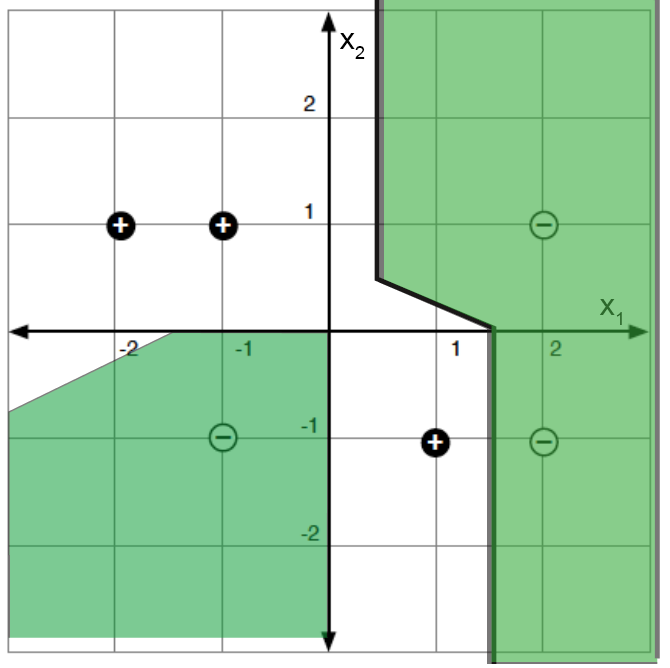
\includegraphics[scale=0.75]{figures/voronoi.png}
\end{center}
In each region, we predict the associated $y$ value.
\question{Convince yourself that these boundaries do represent the
  nearest-neighbor classifier derived from these six data points.}

There are several useful variations on this method.  In {\em
    $k$-nearest-neighbors}, we find the $k$  training points nearest to
the query point $x$ and output the majority $y$ value for
classification or the average for regression.  We can also do {\em
    locally weighted regression} in which we fit locally linear
regression models to the $k$ nearest points, possibly giving less
weight to those that are farther away.  In large data-sets, it is
important to use good data structures (e.g., ball trees) to perform
the nearest-neighbor look-ups efficiently (without looking at all the
data points each time).

\section{Tree Models}
\label{sec-np_trees}

The idea here is that we would like to find a partition of the input
space and then fit very simple models to predict the output in each
piece.  The partition is described using a (typically binary)
``tree'' that recursively splits the space.

\medskip
Tree methods differ by:
\begin{itemize}
  \item The class of possible ways to split the space at each node;
        these are typically linear splits, either aligned with the axes of
        the space, or sometimes using more general classifiers.
  \item The class of predictors within the partitions; these are often
        simply constants, but may be more general classification or
        regression models.
  \item The way in which we control the complexity of the hypothesis: it
        would be within the capacity of these methods to have a separate
        partition element for each individual training example.
  \item The algorithm for making the partitions and fitting the models.
\end{itemize}

One advantage of tree models is that they are easily interpretable by
humans.  This is important in application domains, such as medicine,
where there are human experts who often ultimately make critical
decisions and who need to feel confident in their understanding of
recommendations made by an algorithm. Below is an example decision
tree, illustrating how one might be able to understand the
decisions made by the tree.
\medskip

\begin{examplebox}{\bf Example:}
  Here is a sample tree (reproduced from Breiman, Friedman, Olshen, Stone (1984)):

  \tikzstyle{vertex}=[draw,fill=black!15,rectangle,minimum size=20pt,inner sep=6pt]
  \tikzstyle{leafgreen}=[draw,fill=green!15,rectangle,minimum size=20pt,inner sep=6pt]
  \tikzstyle{leafred}=[draw,fill=red!15,rectangle,minimum size=20pt,inner sep=6pt]

  \begin{center}
    \begin{tikzpicture}[very thick,level distance=2.05cm,level 1/.style={sibling distance=40mm},level 2/.style={sibling distance=5cm}]
      \node [vertex] (r){\begin{minipage}{14em}{\begin{center}Minimum systolic blood pressure over 24h period $\geq$ 91?\end{center}}\end{minipage}}
      child {
          node [leafred] (a) {high risk}
          edge from parent node[left,draw=none,xshift=-0.4pt,yshift=3pt] {no}
        }
      child {
          node [vertex] {Age $\geq$ 65?}
          child {
              node [leafgreen] {low risk}
              edge from parent node[left,draw=none,xshift=-0.4pt,yshift=3pt] {no}
            }
          child {
              node [vertex] {\begin{minipage}{9em}{\begin{center}Is sinus tachycardia present?\end{center}}\end{minipage}}
              child {node [leafgreen] {low risk}
                  edge from parent node[left,draw=none,xshift=-0.4pt,yshift=3pt] {no}
                }
              child {node [leafred] {high risk}
                  edge from parent node[right,draw=none,xshift=-0.0pt,yshift=2pt] {yes}
                }
              edge from parent node[right,draw=none,xshift=-0.0pt,yshift=2pt] {yes}
            }
          edge from parent node[right,draw=none,xshift=-0.0pt,yshift=2pt] {yes}
        };
    \end{tikzpicture}
  \end{center}

\end{examplebox}

These methods are most appropriate for domains where the input space
is not very high-dimensional and where the individual input features
have some substantially useful information individually or in small
groups.  Trees would not be good for image input, but might
be good in cases with, for example, a set of meaningful measurements
of the condition of a patient in the hospital, as in the example
above.

We'll concentrate on the CART/ID3 (``classification and regression
trees'' and ``iterative dichotomizer 3'', respectively) family of
algorithms, which were invented independently in the statistics and
the artificial intelligence communities.  They work by greedily
constructing a partition, where the splits are {\em axis aligned} and
by fitting a {\em constant} model in the leaves.  The interesting
questions are how to select the splits and how to control complexity.
The regression and classification versions are very similar.

As a concrete example, consider the following images:
\begin{center}
  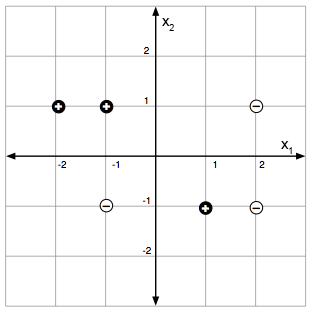
\includegraphics[scale=1]{figures/dt_points.png}
  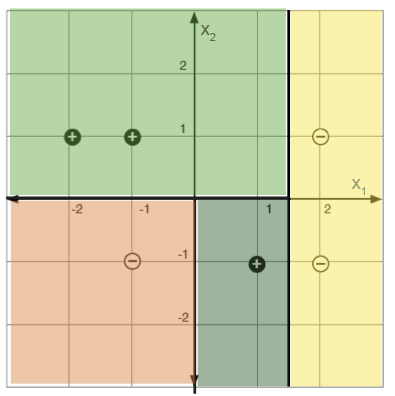
\includegraphics[scale=1]{figures/dt_soln.png}
\end{center}
The left image depicts a set of labeled data points in a two-dimensional
feature space. The right shows a partition into regions by a decision
tree, in this case having no classification errors in the final
partitions.


\subsection{Regression}\index{tree models!regression tree}

\def\Rfeat{R}
\def\Rdata{\hat{R}}

The predictor is made up of
\begin{itemize}
  \item a partition function, $\pi$, mapping elements of the input space into
        exactly one of $M$ regions, $\Rfeat_1, \ldots, \Rfeat_M$, and
  \item a collection of $M$ output values, $O_m$, one for each region.
\end{itemize}

If we already knew a division of the space into regions, we would set
$O_m$, the constant output for region $\Rfeat_m$, to be the average of
the training output values in that region.
For a training data set $\data = \left\{\left(\ex{x}{i},
  \ex{y}{i}\right)\right\}, i = 1, \ldots n$, we let ${\emph I}$ be an indicator
set of all of the elements within $\data$, so that ${\emph I} = \{1, \ldots, n\}$ for
our whole data set.
We can define ${\emph I}_m$ as the subset of data set samples that are
in region $R_m$, so that ${\emph I}_m = \{ i \mid \ex{x}{i} \in R_m\}$. Then
$$O_m = {\rm average}_{i \in {\emph I}_m}~\ex{y}{i}\;\;.$$
We can define the error in a region as $E_m$. For example,
$E_m$ as the sum of squared error would be expressed as
\begin{equation}
  E_m = \sum_{i \in {\emph I}_m}(\ex{y}{i} - O_m)^2\;\;.
\end{equation}
Ideally, we would select the partition to minimize
\begin{equation}
  \lambda M + \sum_{m=1}^M E_m\;\;,
\end{equation}
for some regularization constant $\lambda$.  It is enough to search over all
partitions of the training data (not all partitions of the input
space!) to optimize this, but the problem is NP-complete.
\question{Be sure you understand why it's enough to consider all
  partitions of the training data, if this is your objective.}

\subsubsection{Building a tree}\index{tree models!building a tree}
So, we'll be greedy.  We establish a criterion, given a set of data,
for finding the best single split of that data, and then apply it
recursively to partition the space.  For the discussion below, we
will select the partition of
the data that {\em minimizes the sum of the sum of squared errors of
    each partition element.} Then later, we will consider other
splitting criteria.

Given a data set $\data = \left\{\left(\ex{x}{i},
  \ex{y}{i}\right)\right\}, i = 1, \ldots n$, we now consider ${\emph I}$ to be an indicator
of the subset of elements within $\data$ that we wish to build a tree (or subtree) for.
That is, ${\emph I}$ may already indicate a subset of data set $\data$, based on
prior splits in constructing our overall tree. We define terms as follows:

%% \note{A small subtlety: $\Rdata^+_{j,s}$ is a subset of data, but $\Rfeat_m$ is a partition of the feature space.}

\begin{itemize}
  \item ${\emph I}^+_{j,s}$ indicates the set of examples (subset of
        ${\emph I}$) whose feature value in dimension $j$ is greater than or
        equal to split point $s$;
  \item ${\emph I}^-_{j,s}$ indicates the set of examples (subset of
        ${\emph I}$) whose feature value in dimension $j$ is less than $s$;
  \item $\hat{y}^+_{j,s}$ is the average $y$ value of the data points
        indicated by set ${\emph I}^+_{j,s}$; and
  \item $\hat{y}^-_{j,s}$ is the average $y$ value of the data points
        indicated by set ${\emph I}^-_{j,s}$.
\end{itemize}

Here is the pseudocode. In what follows, $k$ is the largest leaf
size that we will allow in the tree, and is a hyperparameter of the algorithm.
\begin{codebox}
  \Procname{$\proc{BuildTree}({\emph I}, k)$}
  \li  \If $|{\emph I}| \leq k$
  \Then
  \li    Set $\hat{y} = {\rm average}_{i \in {\emph I}}~\ex{y}{i}$
  \li    \Return $\proc{Leaf}({\rm value} = \hat{y})$
  \li  \Else
  \li   \For each split dimension $j$ and split value $s$
  \li     \Do
  Set ${\emph I}^+_{j,s} = \{i \in {\emph I} \mid x_j^{(i)} \geq s\}$
  \li Set ${\emph I}^-_{j,s} = \{i \in {\emph I} \mid x_j^{(i)} < s\}$
  \li Set $\hat{y}^+_{j,s} = {\rm average}_{i \in {\emph I}^+_{j,s}} ~ \ex{y}{i}$
  \li Set $\hat{y}^-_{j,s} = {\rm average}_{i \in {\emph I}^-_{j,s}} ~ \ex{y}{i}$
  \li Set $E_{j,s} = \sum_{i \in {\emph I}^+_{j,s}} (\ex{y}{i} - \hat{y}^+_{j,s})^2 +
    \sum_{i \in {\emph I}^-_{j,s}} (\ex{y}{i} - \hat{y}^-_{j,s})^2$
  \End
  \li        Set $(j^*, s^*) = {\rm arg~min}_{j,s} E_{j,s}$
  \End
  \li    \Return $\proc{Node}(j^*, s^*, \proc{BuildTree}({\emph I}^-_{j^*, s^*}, k), \proc{BuildTree}({\emph I}^+_{j^*, s^*}, k))$
\end{codebox}

In practice, we typically start by calling $\proc{BuildTree}$ with the first
input equal to our
whole data set (that is, with ${\emph I} = \{1,\ldots,n\}$). But then that
call of $\proc{BuildTree}$ can recursively lead to many other calls
of $\proc{BuildTree}$.

Let's think about how long each call of $\proc{BuildTree}$ takes to
run. We have to consider all possible splits. So we consider a split
in each of the $d$ dimensions. In each dimension, we only need to
consider splits betwee two data points (any other split will give the
same error on the training data). So, in total, we consider $O(d n)$
splits in each call to $\proc{BuildTree}$.
\question{Concretely, what would
  be a good set of split-points to consider for dimension $j$ of a
  data set indicated by ${\emph I}$?}

\subsubsection{Pruning}\index{tree models!pruning}
It might be tempting to regularize by using a somewhat large
value of $k$, or by stopping when splitting a node does not significantly
decrease the error.  One problem with short-sighted stopping criteria
is that they might not see the value of a split that will require one
more split before it seems useful.
\question{Apply the decision-tree algorithm to the XOR problem in two
  dimensions.  What is the training-set error of all possible
  hypotheses based on a single split?}
So, we will tend to build a tree that is too large, and then prune it
back.

We define {\em cost complexity}\index{tree models!cost complexity} of a
tree $T$, where $m$ ranges over its leaves, as
\begin{equation}
  C_\alpha(T) = \sum_{m = 1}^{|T|} E_m(T) + \alpha |T|\;\;,
\end{equation}
and $|T|$ is the number of leaves.
For a fixed $\alpha$, we can find a $T$ that (approximately) minimizes
$C_\alpha(T)$ by ``weakest-link'' pruning:
\begin{itemize}
  \item Create a sequence of trees by successively removing the
        bottom-level split that minimizes the increase in overall error,
        until the root is reached.
  \item Return the $T$ in the sequence that minimizes the cost complexity.
\end{itemize}
We can choose an appropriate $\alpha$ using cross validation.

\subsection{Classification}\index{tree models!classification}

The strategy for building and pruning classification trees is very
similar to the strategy for regression trees.

Given a region $\Rfeat_m$ corresponding to a leaf of the tree, we would
pick the output class $y$ to be the value that exists most frequently
(the {\em majority value}) in the data points whose $x$ values are in
that region, i.e., data points indicated by ${\emph I}_m$:
$$O_m = {\rm majority}_{i \in {\emph I}_m}~\ex{y}{i}\;\;.$$
Let's now define the error in a region as the number of data points that do not
have the value $O_m$:
$$E_m = \left|\{i \mid i \in {\emph I}_m \;\text{and}\; \ex{y}{i} \not
  = O_m\}\right|\;\;.$$
We define the {\em empirical probability}\index{empirical probability} of an item from class $k$
occurring in region $m$ as:
\[\hat{P}_{m,k} = \hat{P}({\emph I}_m,k) = \frac{\left|\{i \mid i \in {\emph I}_m
    \;\text{and}\; \ex{y}{i} = k\}\right|}{N_m}\;\;,\] where
$N_m$ is the number of training points in region $m$; that is, $N_m = |{\emph I}_m|.$
For later use, we'll also define the empirical probabilities of split values,
$\hat{P}_{m,j,s}$, as the fraction of points with dimension $j$ in
split $s$ occurring in region $m$ (one branch of the tree), and $1 -
  \hat{P}_{m,j,s}$ as the complement (the fraction of points in the
other branch).

\paragraph*{Splitting criteria}\index{tree models!splitting criteria}
In our greedy algorithm, we need a way to decide which split to make
next.  There are many criteria that express some measure of the
``impurity'' in child nodes.  Some measures include:
\begin{itemize}
  \item {\em Misclassification error}:\index{tree models!splitting criteria!misclassification error}
        \begin{equation}
          Q_m(T) = \frac{E_m}{N_m} = 1 - \hat{P}_{m,O_m}
        \end{equation}
  \item {\em Gini index}:\index{tree models!splitting criteria!Gini index}
        \begin{equation}
          Q_m(T) = \sum_k \hat{P}_{m,k}(1 - \hat{P}_{m,k})
        \end{equation}
  \item {\em Entropy}: \index{tree models!splitting criteria!entropy}
        \begin{equation}
          Q_m(T) = H({\emph I}_m) = - \sum_k \hat{P}_{m,k} \log_2 \hat{P}_{m,k}
        \end{equation}
        So that the entropy $H$ is well-defined when $\hat{P} = 0$, we will stipulate that $0 \log_2 0 = 0$.
\end{itemize}
These splitting criteria are very similar, and it's not entirely obvious which one is
better.  We will focus on entropy, just to be concrete.

Analogous to how for regression we choose the dimension $j$ and split
$s$ that minimizes the sum of squared error $E_{j,s}$, for
classification, we choose the dimension $j$ and split $s$ that
minimizes the weighted average entropy over the ``child'' data points
in each of the two corresponding splits,
${\emph I}^+_{j,s}$ and ${\emph I}^-_{j,s}$.
We calculate the entropy in each split based on the
empirical probabilities of class memberships in the split, and then
calculate the weighted average entropy $\hat{H}$ as
\begin{align}
  \hat{H} & = \text{(fraction of points in left data set)} \cdot H(I_{j,s}^-) \nonumber                     \\
          & \qquad + \text{(fraction of points in right data set)} \cdot H(I_{j,s}^+) \nonumber             \\
          & = (1-\hat{P}_{m,j,s}) H({\emph I}_{j,s}^{-}) + \hat{P}_{m,j,s} H({\emph I}_{j,s}^{+}) \nonumber \\
          & = \frac{|I^-_{j,s}|}{N_m} \cdot H(I_{j,s}^-) + \frac{|I^+_{j,s}|}{N_m} \cdot H(I_{j,s}^+)\; .
\end{align}
Choosing the split that minimizes the entropy of the children is
equivalent to maximizing the {\em information gain}\index{tree
  models!information gain} of the test $x_j = s$, defined by
\begin{eqnarray}
  \proc{infoGain}(x_j = s, {\emph I}_m) & = & H({\emph I}_m) -
  \left(\frac{|I^-_{j,s}|}{N_m} \cdot H(I_{j,s}^-) + \frac{|I^+_{j,s}|}{N_m} \cdot H(I_{j,s}^+)\right)
\end{eqnarray}

In the two-class case (with labels 0 and 1), all of the splitting criteria mentioned
above have the values
\[
  \begin{cases}
    0.0 & \text{when $\hat{P}_{m,0} = 0.0$} \\
    0.0 & \text{when $\hat{P}_{m,0} = 1.0$}
  \end{cases} \; .
\]
The respective impurity curves are shown below, where $p =
  \hat{P}_{m,0}$; the vertical axis plots $Q_m(T)$ for each of the three
criteria.
\begin{center}
  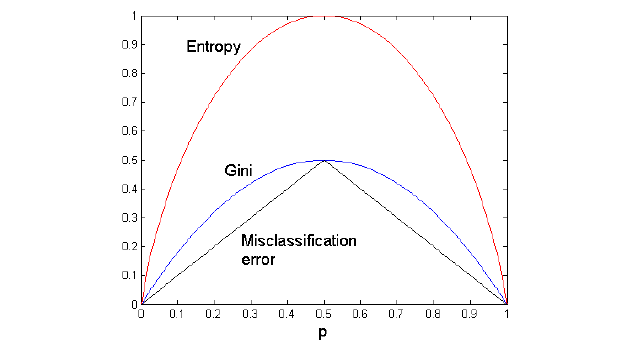
\includegraphics[scale=0.5]{figures/impurity.png}
\end{center}
There used to be endless haggling about which impurity function one should
use.  It seems to be traditional to use {\em entropy} to select which
node to split while growing the tree, and {\em misclassification error}
in the pruning criterion.


\subsection{Bagging}\index{bagging}
\label{sec-np_bagging}

One important limitation or drawback in conventional trees is
that they can have high estimation error: small changes in the data
can result in very big changes in the resulting tree.

  {\em Bootstrap aggregation} is a technique for reducing the estimation
error of a non-linear predictor, or one that is adaptive to the
data. The key idea applied to trees, is to build multiple
trees with different subsets of the data, and then create an ensemble
model that combines the results from multiple trees to make a
prediction.

\begin{itemize}
  \item Construct $B$ new data sets of size $n$. Each data set
        is constructed by sampling $n$ data points with replacement from $\data$.
        A single data set is called {\em bootstrap sample} of $\data$.
  \item Train a predictor $\hat{f}^b(x)$ on each bootstrap sample.
  \item {\em Regression case}:  bagged predictor is
        \begin{equation}
          \hat{f}_{\rm bag}(x) = \frac{1}{B} \sum_{b=1}^B \hat{f}^b(x) \; .
        \end{equation}

  \item {\em Classification case}:  Let $K$ be the number of classes. We
        find a majority bagged predictor as follows. We let
        $\hat{f}^b(x)$ be a ``one-hot'' vector with a single 1 and $K-1$ zeros,
        and define the predicted output $\hat{y}$ for predictor $f^b$ as
        $\hat{y}^b(x) = \argmax{k} \hat{f}^b(x)_k$.  Then
        \begin{equation}
          \hat{f}_{\rm bag}(x) = \frac{1}{B} \sum_{b=1}^B \hat{f}^b(x),
        \end{equation}
        which is a vector containing the proportion of classifiers that
        predicted each class $k$ for input $x$. Then the overall predicted output is
        \begin{equation}
          \hat{y}_{\rm bag}(x) = \argmax{k} \hat{f}_{\rm bag}(x)_k\;\;.
        \end{equation}

        % Alternatively, we can average the class probabilities from the
        % individual classifier, which gives us an even lower-variance estimate.
\end{itemize}

There are theoretical arguments showing that bagging does, in fact,
reduce estimation error.  However, when we bag a model, any simple
intrepetability is lost.
% In the case of regression and {\em squared error}, we can show that
% expected squared error of a classifier trained on a single data set of
% size $n$ is bounded below by the squared error of a classifier that is
% an average over classifiers trained on infinitely many data sets of
% size $n$ {\em drawn from the population}.  This suggests that bagging
% (in which new training sets are drawn from the data set, not
% population) will also decrease error.

% For classification under 0-1 loss, bagging can improve a good
% classifier, but it can also make a bad classifier worse.  
% But, here's a way to understand its advantage:\note{From Dietterich,
%   via Hastie, Tibshirani, and Friedman.}
% \begin{itemize}
% \item Let the Bayes optimal decision at $x$ be $Y(x) = 1$ in a
%   two-class example.
% \item Suppose each ``committee member'' $Y_b$ has an error rate $e_b <
% e < 0.5$ 
% \item Let $S_1(x) = \sum_{b=1}^B I(G_b(x) = 1)$ be the number of votes
%   for class 1 given input $x$
% \item If the committee members are independent, $S_1(x) \sim {\rm
%     Bin}(B, 1-e)$ and so $\Pr(S_1 > B/2) \rightarrow 1$ as $B$ gets large.
% \note{This is the ``Wisdom of Crowds.''}
% \end{itemize}
% The main issue with this analysis is that it assumes the committee
% members are independent, which they definitely are not in this
% case.


\subsection{Random Forests}

Random forests are collections of trees that are constructed to be
de-correlated, so that using them to vote gives maximal advantage.
In competitions, they often have excellent classification performance
among large collections of much fancier methods.

In what follows, $B$, $m$, and $n$ are hyperparameters of the algorithm.

\begin{codebox}
  \Procname{$\proc{RandomForest}(\data; B, m, n)$}
  \li  \For $b = 1, \ldots, B$
  \Do
  \li    Draw a bootstrap sample $\data_b$ of size $n$ from $\data$
  \li    Grow a tree $T_b$ on data $\data_b$ by recursively:
  \Do
  \li      Select $m$ variables at random from the $d$ variables
  \li      Pick the best variable and split point among the $m$ variables
  \li      Split the node
  \End
  \End
  \li   \Return tree $T_b$
\end{codebox}
Given the ensemble of trees, vote to make a prediction on a new $x$.

\subsection{Tree variants and tradeoffs}

There are many variations on the tree theme. One is to employ
different regression or classification methods in each leaf.  For
example, a linear regression might be used to model the examples in
each leaf, rather than using a constant value.

In the relatively simple trees that we've considered, splits
have been based on only a single feature at a time, and with the
resulting splits being axis-parallel. Other methods for splitting are
possible, including consideration of multiple features and linear
classifiers based on those, potentially resulting in non-axis-parallel
splits. Complexity is a concern in such cases, as many possible
combinations of features may need to be considered, to select the
best variable combination (rather than a single split variable).

Another generalization is a {\em hierarchical mixture of experts},
where we make a ``soft'' version of trees, in which the splits are
probabilistic (so every point has some degree of membership in every
leaf). Such trees can be trained using a form of gradient
descent. Combinations of bagging, boosting, and mixture tree
approaches (e.g., {\em gradient boosted trees}) and
implementations are readily available (e.g., XGBoost).

Trees have a number of strengths, and remain a valuable tool
in the machine learning toolkit.  Some benefits include being
relatively easy to interpret, fast to train, and ability to handle
multi-class classification in a natural way. Trees can easily
handle different loss functions; one just needs to change the
predictor and loss being applied in the leaves. Methods also exist to
identify which features are particularly important or influential in
forming the tree, which can aid in human understanding of the data
set.  Finally, in many situations, trees perform surprisingly
well, often comparable to more complicated regression or
classification models. Indeed, in some settings it is considered good
practice to start with trees (especially random forest or
boosted trees) as a ``baseline'' machine learning model,
against which one can evaluate performance of more sophisticated
models.



%%%%%%%%%%%%%%%%%%%%%%%%%%%%%%%%%%%%%%%%%%%%%%%%%%%%%%%%%%%%%%%%%%%%%%%%%%%%%





%%% Local Variables:
%%% mode: latex
%%% TeX-master: "top"
%%% End:
